%\modeCorrection

%%%% début de la page
\renewcommand{\thesection}{\textcolor{red}{Partie \Roman{section} -}}
\renewcommand{\thesubsection}{\textcolor{red}{\Roman{section}.\arabic{subsection}}}
\renewcommand{\thesubsubsection}{\textcolor{red}{\Roman{section}.\arabic{subsection}.\alph{subsubsection}}}

\setcounter{section}{0}
\setcounter{document}{0}
\sndEnTeteTPOnze

\begin{center}
\begin{mdframed}[style=titr, leftmargin=60pt, rightmargin=60pt, innertopmargin=7pt, innerbottommargin=7pt, innerrightmargin=8pt, innerleftmargin=8pt]

\begin{center}
\large{\textbf{TP 11 : L'\oe il, un instrument remarquable
}}
\end{center}
\end{mdframed}
\end{center}


%%%% objectifs
\begin{tcolorbox}[colback=blue!5!white,colframe=blue!75!black,title=Objectifs de la séance :]
\begin{itemize}
    \item Modéliser l'\oe il ;
    \item Produire et caractériser l'image réelle d'un objet plan réel formée par une lentille mince convergente ;
    \item Utiliser le théorème de Thalès ;
\end{itemize}
\end{tcolorbox}

%%%% Consignes
\begin{tcolorbox}[colback=red!5!white,colframe=red!75!black,title= Consignes :]
\begin{itemize}
    \item Faire attention au matériel lors de son utilisation ;
\end{itemize}
\end{tcolorbox}

%%%% contexte
\section{Analyse documentaire}
\begin{tcolorbox}[colback=orange!5!white,colframe=orange!75!black,title= C'est pas sorcier l'\oe il ! :]
Regarder la vidéo tirée de l'émission \og C'est pas Sorcier \fg~ à l'adresse suivante \url{https://ladigitale.dev/digiview/#/v/6576d364e2055} ou en scannant le QR-code : 
\begin{center}
    
\includegraphics[scale=0.4]{Images/CPasSorcier_Oeil.png}
\end{center}
Compléter le tableau suivant :
\begin{center}
    \begin{tabular}{|C{0.3}|C{0.3}|C{0.3}|}
    \hline
        \cellcolor{orange!25} \oe il & \cellcolor{orange!25} appareil photo & \cellcolor{orange!25} rôle \\
        \hline
        Cornée & %Lentille  
        & %Faire converger la lumière dans l'\oe il 
        \\
        \hline
        Iris & %Diaphragme 
        & %Faire passer plus ou moins de lumière dans l'\oe il 
        \\
        \hline 
        Cristallin & %Lentille 
        &%Faire converger la lumière sur la rétine
        \\
        \hline 
        Rétine & %Pélicule
        & %Reçoit la lumière/ Convertir le signal lumineux en signal électrique pour le cerveau 
        \\
        \hline 
    \end{tabular}
\end{center}

\problematique{Comment se propage la lumière à travers une lentille ? Quelle dimension a l'image d'un objet réel à travers une lentille convergente ?}
\end{tcolorbox}


\begin{mdframed}[style=autreexo]
\textbf{\bsc{Liste du matériel}}
\vspace{-0.5cm}
\begin{multicols}{2}
\begin{itemize}
    \item Une \og laser box \fg ;
    \item Des lentilles convergentes ;
    \item Un tableau magnétique ;
\end{itemize}
\end{multicols}
\end{mdframed}

%%%% documents

%%%%
\section{Propriétés des lentilles convergentes}

\subsection{Mise en évidence de 3 points particuliers}

\question{Observer sur le tableau magnétique le cheminement d'un rayon lumineux passant par le \textbf{centre de la lentille} aussi appelé \textcolor{red}{centre optique} et noté O.\\

\textit{Observations :} \texteTrouMultiLignes{Lorsqu'un rayon lumineux passe par le centre optique de la lentille, il \underline{n'est pas dévié}.}{1}
\begin{center}
    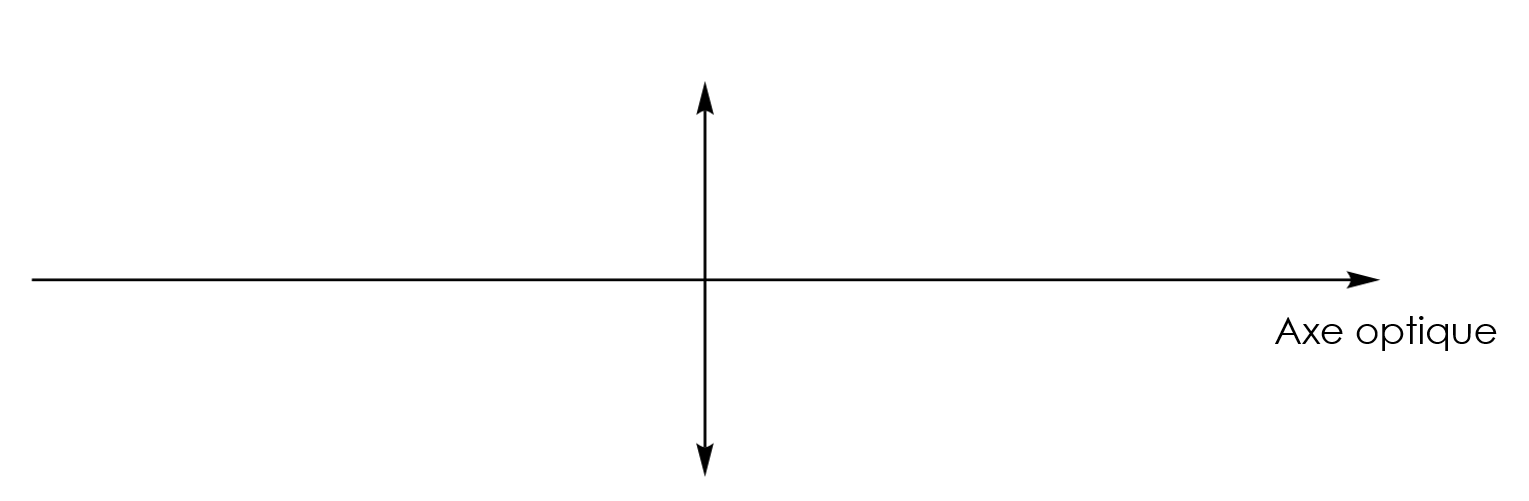
\includegraphics[scale=0.6]{Images/Lentille_construction.PNG}
\end{center}
}{\begin{center}
    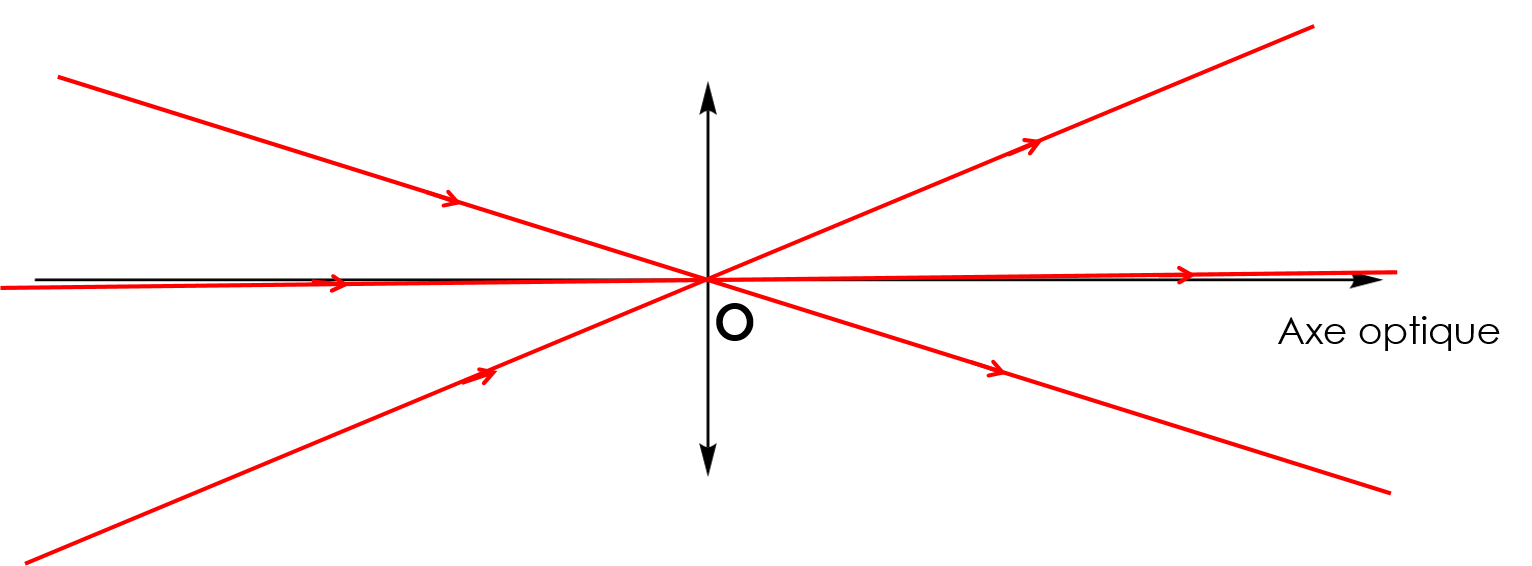
\includegraphics[scale=0.5]{Images/Lentille_construction_centreoptique.png}
\end{center}}{0}

\question{Observer sur le tableau magnétique le cheminement de rayons lumineux \textbf{arrivant parallèles à l'axe optique}.\\

\textit{Observations :} \texteTrouMultiLignes{Lorsqu'un rayon lumineux arrive parallèlement à l'axe optique, il ressort sur un point particulier appelé  \underline{foyer focal image}, noté F'.}{1}
\begin{center}
    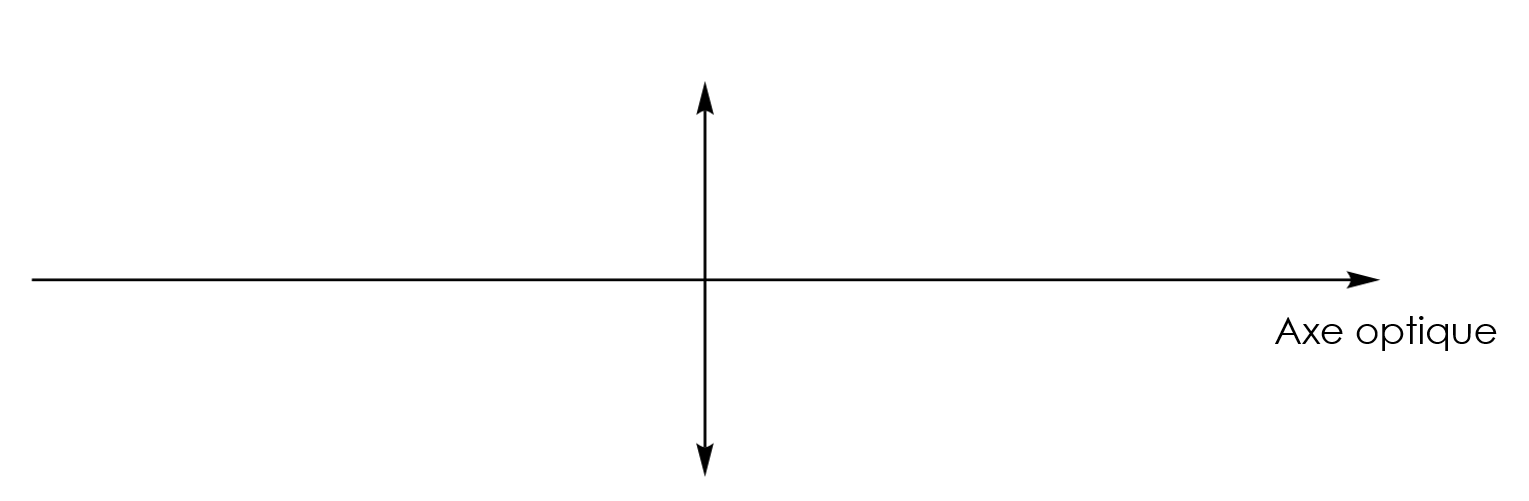
\includegraphics[scale=0.6]{Images/Lentille_construction.PNG}
\end{center}
}{\begin{center}
    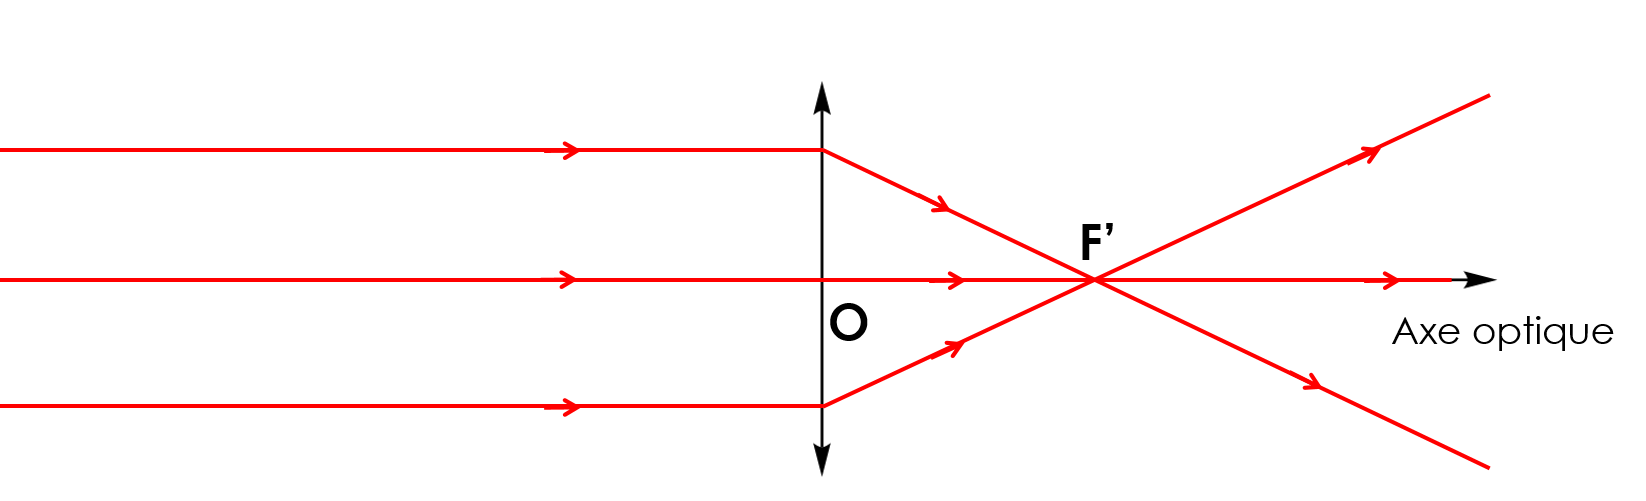
\includegraphics[scale=0.5]{Images/Lentille_construction_foyerimage.png}
\end{center}}{0}

\question{Observer sur le tableau magnétique le cheminement de rayons lumineux \textbf{émergeant parallèles à l'axe optique}.\\

\textit{Observations :} \texteTrouMultiLignes{Lorsqu'un rayon lumineux émerge parallèle à l'axe optique, il provient d'un point particulier appelé \underline{foyer focal objet}, noté F.}{2}
\begin{center}
    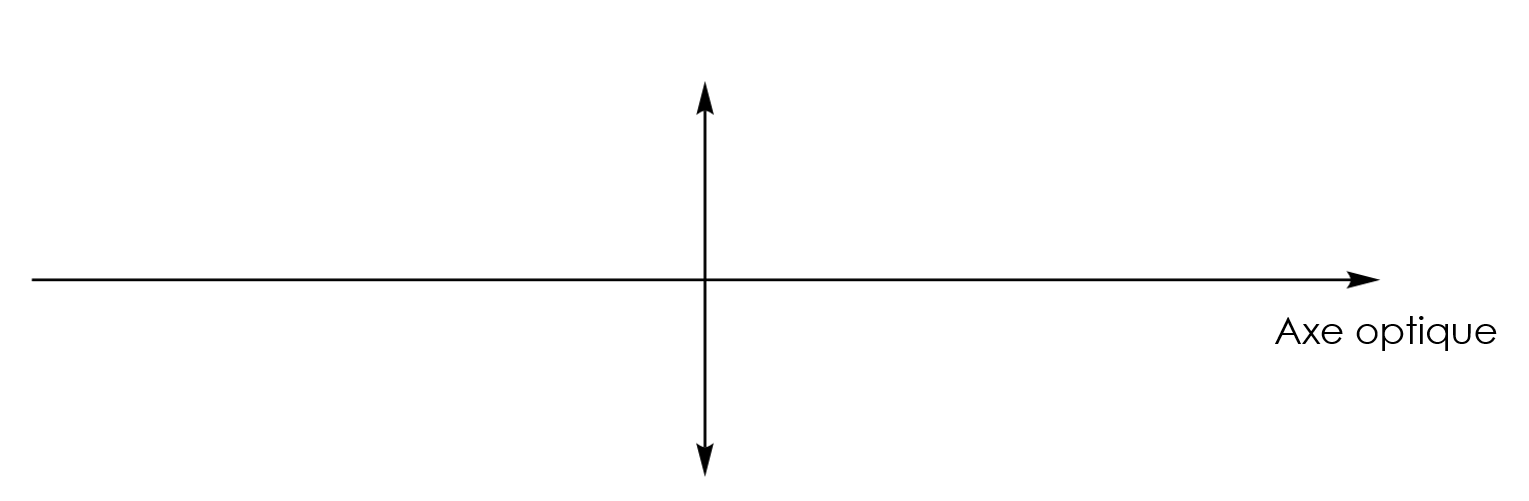
\includegraphics[scale=0.6]{Images/Lentille_construction.PNG}
\end{center}
}{\begin{center}
    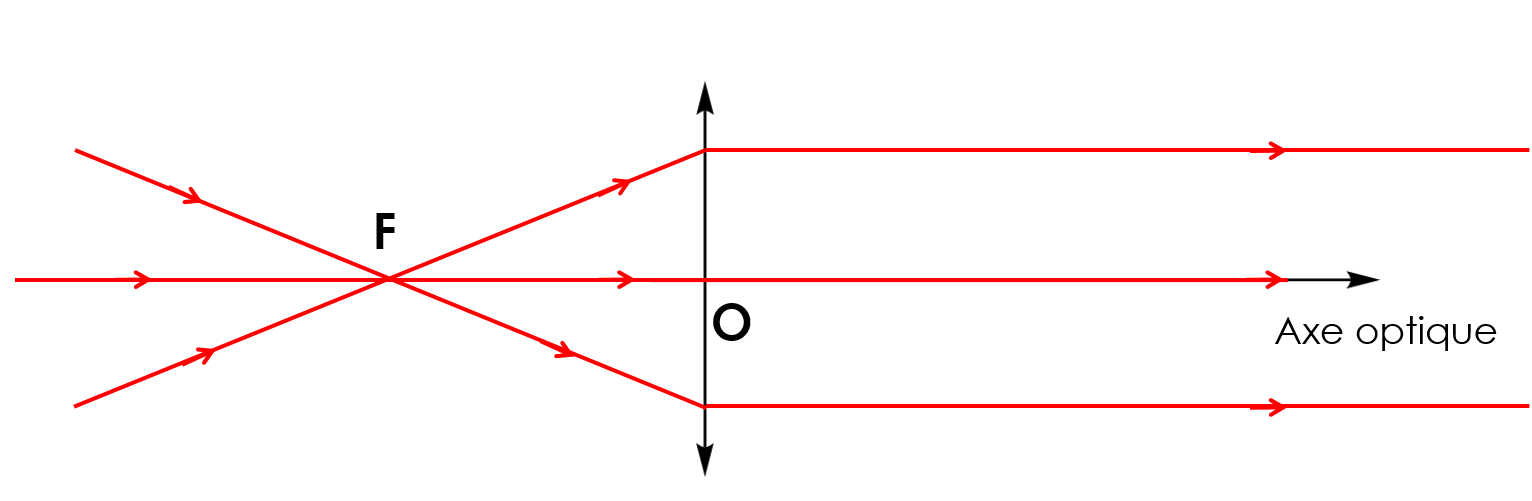
\includegraphics[scale=0.5]{Images/Lentille_construction_foyerobjet.png}
\end{center}}{0}

\subsection{\`{A} retenir}

\begin{multicols}{2}
\begin{tcolorbox}[colback=green!5!white,colframe=green!75!black,title=\textbf{Lentille convergente :}]  
    Une lentille est caractérisée par son \textcolor{red}{centre optique} O par lequel passe l'axe optique, son \textcolor{red}{foyer image} F' et \textcolor{red}{son foyer objet} F.
\end{tcolorbox}
\begin{tcolorbox}[colback=red!5!white,colframe=red!75!black,title=\textbf{Propriété sur F et F' :}]
Les foyers objets F et images F' sont \textcolor{red}{symétriques} par rapport au centre optique O de la lentille.
\end{tcolorbox}

\end{multicols}
    \begin{tcolorbox}[colback=red!5!white,colframe=red!75!black,title=\textbf{Règles de construction d'une image par une lentille :}]
\begin{itemize}
    \item Le rayon passant par le centre optique O \textbf{n'est pas dévié} ;
    \item Les rayons arrivant parallèlement à l'axe optique \textbf{ressortent sur le foyer image F'} ;
    \item Les rayons passant par le foyer objet F \textbf{ressortent parallèle à l'axe optique $\Delta$}.
\end{itemize}
\end{tcolorbox}
\newpage
\section{Image d'un objet plan à travers une lentille convergente}
\setcounter{exercice}{0}

\begin{mdframed}[style=autreexo]
\textbf{\bsc{Liste du matériel}}
\vspace{-0.5cm}
\begin{multicols}{2}
\begin{itemize}
    \item Une source de lumière avec un objet plan ;
    \item Une lentille convergentes de distance focale OF'=f'=12,5~cm (8 dioptries) ;
    \item Un banc optique ;
    \item Un écran recouvert d'un papier millimétré;
\end{itemize}
\end{multicols}
\end{mdframed}

\begin{doc}{Protocole expérimental}
\begin{center}
    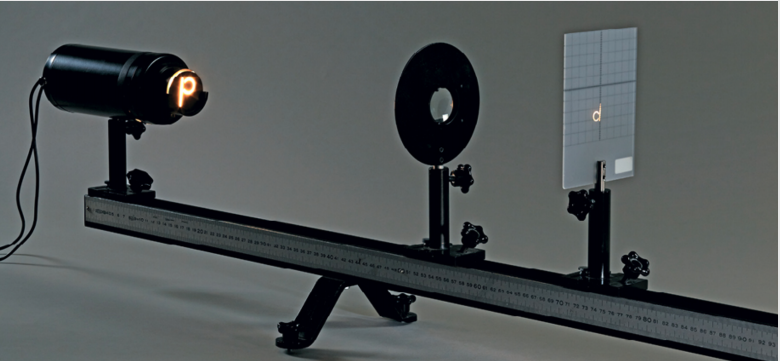
\includegraphics[scale=0.7]{Images/Protocole_lentille.PNG}
\end{center}
   \begin{enumerate}
       \item Réaliser le montage ci-dessus ;
       \item Mesurer la taille de l'objet lumineux AB ;
       \item Placer la lentille convergente à différentes distances de l'objet lumineux et mesurer la distance entre l'objet et la lentille OA à l'aide du banc optique ;
       \item Déplacer l’écran pour observer une \textbf{image nette} sur l’écran ;
       \item Mesurer la distance entre la lentille et l'écran notée $\overline{\text{OA'}}$ ;
       \item Mesurer la taille $\overline{\text{A'B'}}$ de l'image sur l'écran ;
   \end{enumerate}
\end{doc}

\begin{tcolorbox}[colback=green!5!white,colframe=green!75!black,title=\textbf{Définition du grandissement :}]  
    On appelle \textcolor{red}{grandissement}, noté $\gamma$, le rapport entre la taille \textcolor{red}{algébrique} de l'image $\overline{\text{A'B'}}$ et celle de l'objet $\overline{\text{AB}}$ :
    \begin{equation*}
        \gamma = \frac{\overline{\text{A'B'}}}{\overline{\text{AB}}}
    \end{equation*}
    \begin{itemize}
    \item Si $\gamma$ est négatif, alors l'image est renversée ;
    \item Si $\abs{\gamma}$ est plus petit que 1, alors l'image est plus petite que l'objet.
\end{itemize}
\end{tcolorbox}
\clearpage
%\vspace{-0.5cm}
\question{Mettre en \oe uvre les \textbf{4 premières étapes} protocole expérimental donné dans le document 1 en prenant $\overline{\text{OA}}$ = -30~cm.}{On mesure AB=5cm.}{0}
%\\
\question{Indiquer si l'image est droite ou renversée, agrandie ou rétrécie.}{L'image est renversée et rétrécie.}{0}
%\\
%\clearpage
\question{Compléter le schéma suivant en plaçant l'axe optique, le centre optique O, le foyer focal objet F et le foyer focal image F'. \`{A} l'aide des règes de construction énoncées dans la partie II, tracer les rayons lumineux provenant de B pour construire l'image B' à travers la lentille. 
\begin{center}
    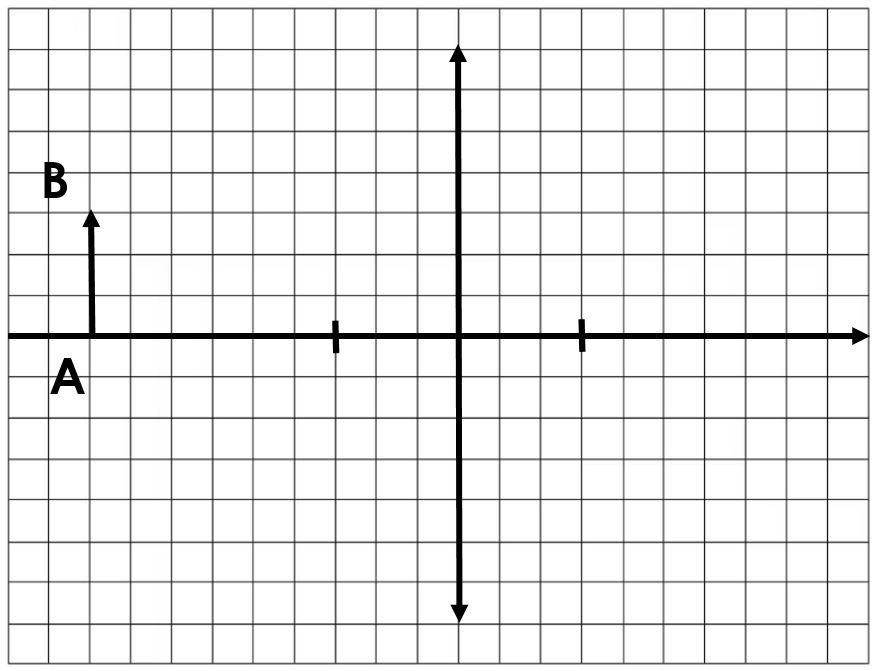
\includegraphics[scale=0.9]{Images/Lentille_construction_papier.png}
\end{center}}{\begin{center}
    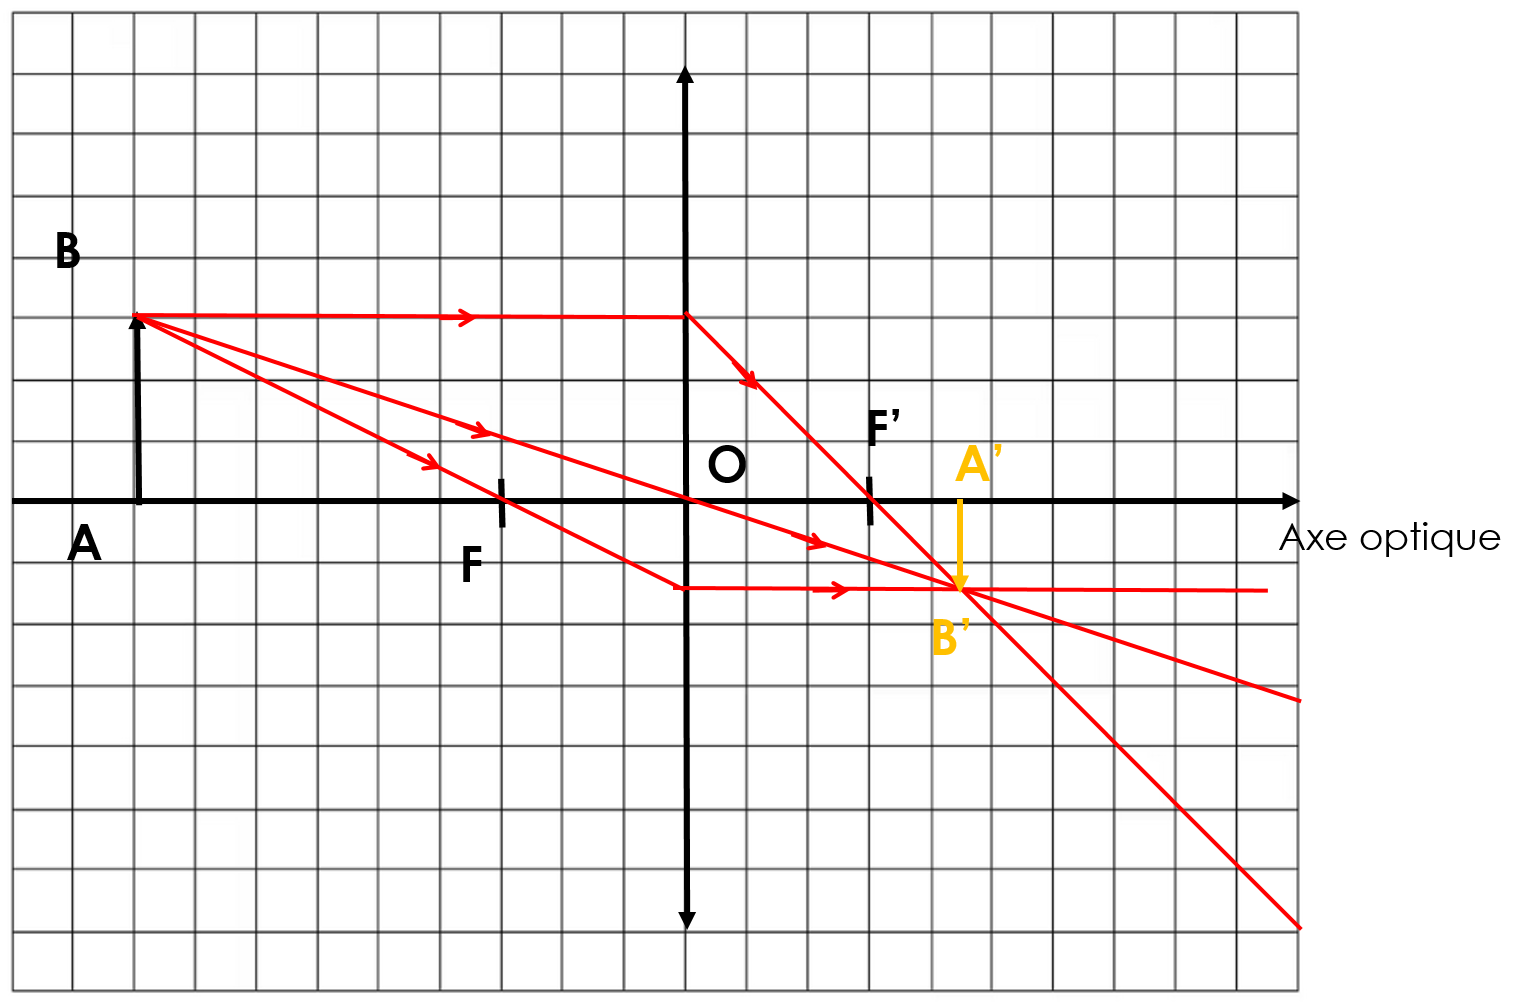
\includegraphics[scale=0.6]{Images/Lentille_construction_papier_correction.png}
\end{center}}{0}
\newpage
\question{Réaliser le protocole du document 1 et compléter le tableau suivant : 
\begin{center}
    \begin{tabular}{|C{0.2}|C{0.15}|C{0.15}|C{0.15}|C{0.15}| }
        \hline 
        \cellcolor{orange!25} Expérience & \cellcolor{blue!25}n$\degree$1 & \cellcolor{blue!25}n$\degree$2 & \cellcolor{blue!25}n$\degree$3 & \cellcolor{blue!25}n$\degree$4\\
         \hline
         \cellcolor{orange!25} Distance $\overline{\text{OA}}$ (en cm) & -15 & -30 & -50 & -60 \\
         \hline
         \cellcolor{orange!25} Distance $\overline{\text{OA'}}$ (en cm) & & & &  \\
         \hline
         \cellcolor{orange!25} Nature de l'image (agrandie ou rétrécie, droite ou renversée) & & & & \\
         \hline
         \cellcolor{orange!25} Taille de l'image $\overline{\text{AB'}}$ (en cm) & & & & \\
         \hline
    \end{tabular}
\end{center}}{\begin{center}
    \begin{tabular}{|C{0.2}|C{0.15}|C{0.15}|C{0.15}|C{0.15}| }
        \hline 
        \cellcolor{orange!25} Expérience & \cellcolor{blue!25}n$\degree$1 & \cellcolor{blue!25}n$\degree$2 & \cellcolor{blue!25}n$\degree$3 & \cellcolor{blue!25}n$\degree$4\\
         \hline
         \cellcolor{orange!25} Distance $\overline{\text{OA}}$ (en cm) & -15 & -30 & -50 & -60 \\
         \hline
         \cellcolor{orange!25} Distance $\overline{\text{OA'}}$ (en cm) & 75 & 21 & 17 & 16 \\
         \hline
         \cellcolor{orange!25} Nature de l'image (agrandie ou rétrécie, droite ou renversée) & Agrandie, renversée & Rétrécie, renversée & Rétrécie, renversée & Rétrécie, renversée\\
         \hline
         \cellcolor{orange!25} Taille de l'image $\overline{\text{AB'}}$ (en cm) & -25 & -3,5 & -1,7 & -1,3 \\
         \hline
    \end{tabular}
\end{center}}{0}

\question{Indiquer comment varie la taille de l'image lorsqu'on rapproche l'objet de la lentille.}{La taille de l'image augmente. On ne peut même plus obtenir d'image nette à partir si OA<12,5cm.}{0}

\question{\`{A} l'aide de vos résultats dans le tableau précédent, compléter le tableau suivant :
\begin{center}
    \begin{tabular}{|C{0.2}|C{0.15}|C{0.15}|C{0.15}|C{0.15}| }
        \hline 
        \cellcolor{orange!25} Expérience & \cellcolor{blue!25}n$\degree$1 & \cellcolor{blue!25}n$\degree$2 & \cellcolor{blue!25}n$\degree$3 & \cellcolor{blue!25}n$\degree$4\\
        \hline
        \cellcolor{orange!25} $\frac{\overline{\text{OA'}}}{\overline{\text{OA}}}$ & & & &  \\
        \hline
        \cellcolor{orange!25} Grandissement $\gamma$ &  &  &  & \\
        \hline 
    \end{tabular}
\end{center}
}{\begin{center}
    \begin{tabular}{|C{0.2}|C{0.15}|C{0.15}|C{0.15}|C{0.15}| }
        \hline 
        \cellcolor{orange!25} Expérience & \cellcolor{blue!25}n$\degree$1 & \cellcolor{blue!25}n$\degree$2 & \cellcolor{blue!25}n$\degree$3 & \cellcolor{blue!25}n$\degree$4\\
        \hline
        \cellcolor{orange!25} $\frac{\overline{\text{OA'}}}{\overline{\text{OA}}}$ & -5 & -0,7 & -0,34 & -0,27 \\
        \hline
        \cellcolor{orange!25} Grandissement $\gamma$ & -5 & -0,7 & -0,34 & -0,27\\
        \hline 
    \end{tabular}
\end{center}}{0}

\question{Proposer une relation entre le grandissement et le rapport $\frac{\overline{\text{OA'}}}{\overline{\text{OA}}}$.}{D'après les mesures expérimentales, on peut conjecturer que $\gamma=\frac{\overline{\text{OA'}}}{\overline{\text{OA}}}$}{0}

\question{\`{A} l'aide du théorème de Thalès dans les triangles OAB et OA'B' (voir la question 6), démontrer la relation conjecturée dans la question précédente.}{Dans les triangles OAB et OA'B', les droites (AB) et (A'B') sont parallèles. On peut dès lors appliquer le théorème de Thalès qui donne les relations suivantes :
\begin{equation*}
    \frac{\overline{\text{OA'}}}{\overline{\text{OA}}} = \frac{\overline{\text{A'B'}}}{\overline{\text{AB}}} = \frac{\overline{\text{OB'}}}{\overline{\text{OB}}}
\end{equation*}
La première égalité donne la relation recherchée.}{0}
%\\

\begin{facile}{\large Simulation sur les lentilles}
\vspace{0.5cm}
\begin{multicols}{2}
\begin{center}
    On aurait pu tout faire à l'aide de ce logiciel de simulation (merci l'université du Colorado !) :

    \url{https://phet.colorado.edu/fr/simulations/geometric-optics-basics}\\
    \vspace{4cm}
    \begin{Large}
        \textbf{Mais c'est quand même bien mieux d'expérimenter en TP, non ??}
    \end{Large}
\end{center}

%\begin{center}
 %   \includegraphics[scale=0.15]{Images/Joyeux_noel_dispersé.png}
%\end{center}
\end{multicols}


\end{facile}
%\newpage
%\papiermillimetre